% Metódy inžinierskej práce

\documentclass[10pt,twoside,slovak,a4paper]{article}

\usepackage[slovak]{babel}
%\usepackage[T1]{fontenc}
\usepackage[IL2]{fontenc} % lepšia sadzba písmena Ľ než v T1
\usepackage[utf8]{inputenc}
\usepackage{graphicx}
\usepackage{url} % príkaz \url na formátovanie URL
\usepackage{hyperref} % odkazy v texte budú aktívne (pri niektorých triedach dokumentov spôsobuje posun textu)

\usepackage{cite}
%\usepackage{times}

\pagestyle{headings}

\title{Kultúrny model pre správanie nehrateľných postav v počítačových hrách\thanks{Semestrálny projekt v predmete Metódy inžinierskej práce, ak\@. rok 2021/22, vedenie cvičení: Ing. Fedor Lehocki, PhD.}} % meno a priezvisko vyučujúceho na cvičeniach

\author{Martin Szabo\\[2pt]
	{\small Slovenská technická univerzita v Bratislave}\\
	{\small Fakulta informatiky a informačných technológií}\\
	{\small \texttt{xszabom5@stuba.sk}}
	}

\date{\small 4.\ október 2021} % upravte

\begin{document}

\maketitle

\begin{abstract}

Počítačové hry sa často snažia čo najbližšie priblížiť realite. Veľa hier sa snaží priblížiť realite práve tým že 
majú realistickú fyziku a grafiku. Ale málo hier sa zaoberá tým ako sa nehrateľné postavy tzv. `NPC' z anglického
`Non-playable character' správajú v hernom svete. Aby sme sa priblížili k realite čo najviac je dôležité aby postavy
dokázali prejavovať emócie, mať osobnostné črty a samozrejme správať sa sociálne aby sme získali dojem že tá postava
myslí a žije aj keď je to len pár pixelov v počítačovej hre. Model ktorým sa tento článok zaoberá ponúka lepšie
možnosti ako modelovať realistickejší vzor správania.

\end{abstract}

\section{Úvod}

Herný priemysel je jeden z najpopulárnejších a najrýchlejšie rastúcich priemyslov.
Tisíce eur sa investujú do rôznych technológií na vývoj hier a panuje tam veľká konkurencia
medzi jednotlivými vývojárskymi firmami. Každý sa snaží mať tú najlepšiu a najpopulárnejšiu
hru v celom priemysle. Tento priemysel je zaplavený rôznymi hrami ktoré pokiaľ chcú zaujať hráčov
tak musia robiť niečo unikátnejšie než ich konkurencia. V tomto článku sa budeme zaoberať témou
kultúrneho modelu nehrateľných postav ktorá je veľakrát podceňovaná. Namodelovanie správnej kultúry
nehrateľných postav hráčom ponúka hlbšie emočné spojenie s postavami v príbehu a pomáha hráčovi
vžiť sa do herného sveta. Existujú hry ktoré simulovali rôzne kultúry ale žiadne to nerobili do takej 
miery ako to vidíme v reálnom svete. Postava ktorá bude namodelovaná cez model predstavený v 
tomto článku bude schopná nie len patriť pod nejakú kultúru ale aj správať sa adekvátne v rámci 
jej kultúrneho modelu. Bude reagovať na zlé a dobré podnety od hráča ale aj od iných nehrateľných 
postáv a bude môcť prejavovať široké spektrum emócií rovnako ako to je aj v realite u ľudí. Taktiež bude 
môcť usúdiť na základe správania hráča a iných nehrateľných postav okolo nej jej vzťah k nim. Tento model
sa bude usilovať o simuláciu reálnej mysle človeka a následne bude z neho vyplývať správanie nehrateľných
postav v hernom svete.

\section{Nejaká časť}\label{nejaka}

Z obr.~\ref{f:rozhod} je všetko jasné. 

\begin{figure*}[tbh]
\centering
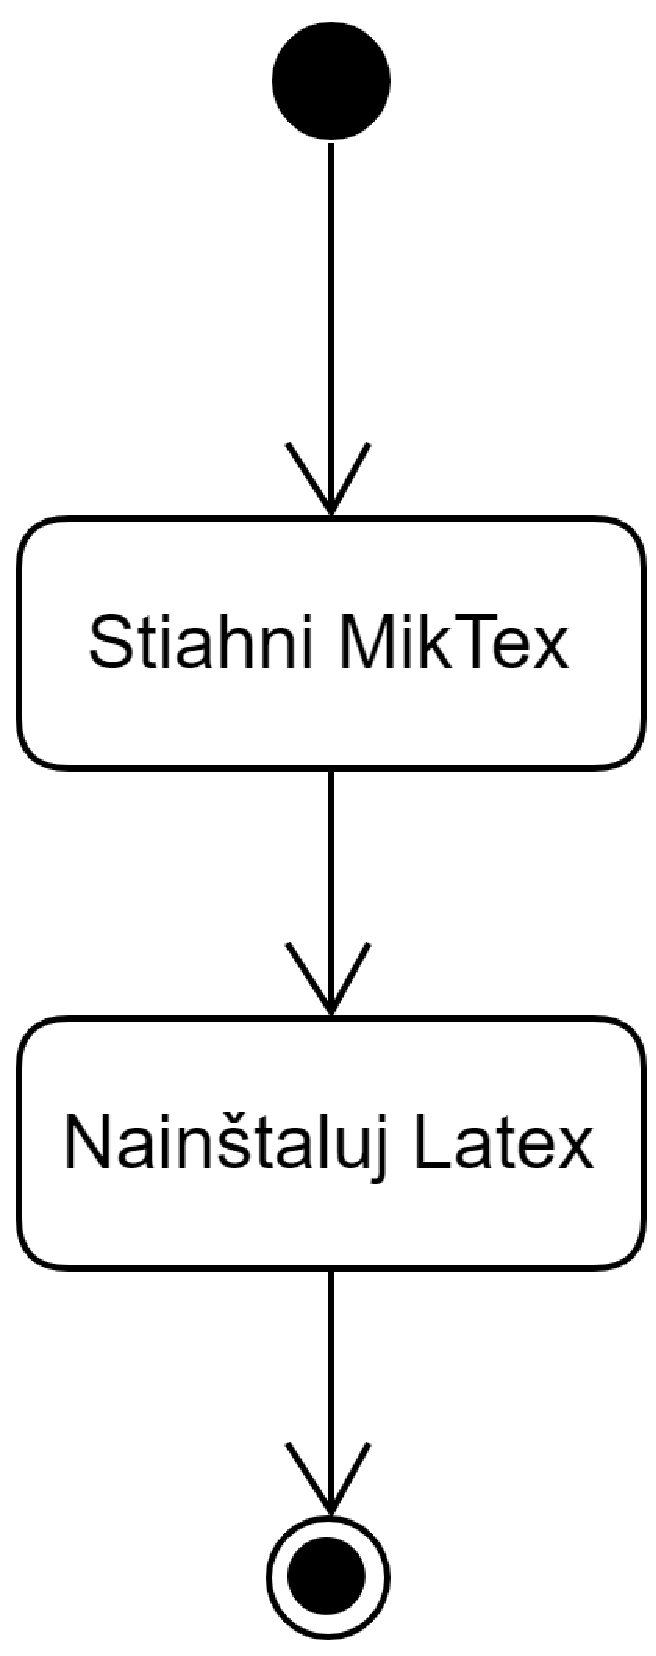
\includegraphics[scale=1.0]{diagram.pdf}
Aj text môže byť prezentovaný ako obrázok. Stane sa z neho označný plávajúci objekt. Po vytvorení diagramu zrušte znak \texttt{\%} pred príkazom \verb|\includegraphics| označte tento riadok ako komentár (tiež pomocou znaku \texttt{\%}).
\caption{Rozhodujúci argument.}\label{f:rozhod}
\end{figure*}

\section{Iná časť}\label{ina}

Základným problémom je teda\ldots{} Najprv sa pozrieme na nejaké vysvetlenie (časť~\ref{ina:nejake}), a potom na ešte nejaké (časť~\ref{ina:nejake}).\footnote{Niekedy môžete potrebovať aj poznámku pod čiarou.}

%Môže sa zdať, že problém vlastne nejestvuje\cite{Coplien:MPD}, ale bolo dokázané, že to tak nie je~\cite{Czarnecki:Staged, Czarnecki:Progress}. Napriek tomu, aj dnes na webe narazíme na všelijaké pochybné názory\cite{PLP-Framework}. Dôležité veci možno \emph{zdôrazniť kurzívou}.
Citácia vyzerá asi takto~\cite{Bicalho2020}
\subsection{Nejaké vysvetlenie}\label{ina:nejake}

Niekedy treba uviesť zoznam:

\begin{itemize}
\item jedna vec
\item druhá vec
	\begin{itemize}
	\item x
	\item y
	\end{itemize}
\end{itemize}

Ten istý zoznam, len číslovaný:

\begin{enumerate}
\item jedna vec
\item druhá vec
	\begin{enumerate}
	\item x
	\item y
	\end{enumerate}
\end{enumerate}

\subsection{Ešte nejaké vysvetlenie}\label{ina:este}

\paragraph{Veľmi dôležitá poznámka.}
Niekedy je potrebné nadpisom označiť odsek. Text pokračuje hneď za nadpisom.

\section{Dôležitá časť}\label{dolezita}

\section{Ešte dôležitejšia časť}\label{dolezitejsia}

\section{Záver}\label{zaver} % prípadne iný variant názvu

%\acknowledgement{Ak niekomu chcete poďakovať\ldots}

% týmto sa generuje zoznam literatúry z obsahu súboru literatura.bib podľa toho, na čo sa v článku odkazujete
\bibliography{literatura}
\bibliographystyle{plain} % prípadne alpha, abbrv alebo hociktorý iný
\end{document}
